\documentclass[conference]{IEEEtran}
%Template version as of 6/27/2024

\usepackage{cite}
\usepackage{amsmath,amssymb,amsfonts}
\usepackage{algorithmic}
\usepackage{graphicx}
\graphicspath{{images/}}
\usepackage{textcomp}
\usepackage{xcolor}
\def\BibTeX{{\rm B\kern-.05em{\sc i\kern-.025em b}\kern-.08em
    T\kern-.1667em\lower.7ex\hbox{E}\kern-.125emX}}
% \setlength{\parindent}{1em}
% \setlength{\parskip}{0.8em}
\begin{document}

\title{Neural Networks for Neural Tumors}

% old author block
% \author{
% \IEEEauthorblockN{\large Joe Vogel}
% \IEEEauthorblockA{\textit{UC Davis Computer Science} \\
% jvogel@ucdavis.edu}

% \and
% \IEEEauthorblockN{\large Nam Nguyen}
% \IEEEauthorblockA{\textit{UC Davis Computer Science} \\
% ncnn@ucdavis.edu}

% \and
% \IEEEauthorblockN{\large Jonathan Mo}
% \IEEEauthorblockA{\textit{UC Davis Computer Science} \\
% jtnmo@ucdavis.edu}

% \and
% \IEEEauthorblockN{\large Aryan Karnwal}
% \IEEEauthorblockA{\textit{UC Davis Computer Science} \\
% akarnwal@ucdavis.edu}

% \and
% \IEEEauthorblockN{\large Richard Ho}
% \IEEEauthorblockA{\textit{UC Davis Computer Science} \\
% rdho@ucdavis.edu}
% }

\author{
\centering
\begin{minipage}[t]{0.9\textwidth}
  \centering
  \begin{tabular}{ccc}
    Joe Vogel & Nam Nguyen & Jonathan Mo \\
    \textit{UC Davis Computer Science} & \textit{UC Davis Computer Science} & \textit{UC Davis Computer Science} \\
    jvogel@ucdavis.edu & ncnn@ucdavis.edu & jtnmo@ucdavis.edu \\
    \vspace{0.6em}
  \end{tabular}
  \begin{tabular}{cc}
    Aryan Karnwal & Richard Ho \\
    \textit{UC Davis Computer Science} & \textit{UC Davis Computer Science} \\
    akarnwal@ucdavis.edu & rdho@ucdavis.edu \\
  \end{tabular}
\end{minipage}
}

\maketitle

\begin{abstract}
This report documents the process of creating a machine learning model that classifies brain tumors using MRI brain scan imagery. This project saw the creation of three successful models using the following algorithms: Convolutional Neural Network, Support Vector Machine, and Random Forest. 
\end{abstract}

\begin{IEEEkeywords}
Brain tumor classification, Convolutional Neural Network (CNN), MRI brain imagery, Random Forest (RF), Support Vector Machine (SVM). 
\end{IEEEkeywords}

\large 
\section{\large Introduction (1-2 pages)}
Hundreds of thousands of MRI brain scans are performed every day. With MRI scans being so intricate, it can sometimes be hard for even a trained professional to determine whether or not a patient has a brain tumor, and even harder to tell which kind. 

\subsection{\large Motivation}
Having a tool that could detect and identify tumors within seconds, and with high accuracy, would save a lot of time and money. Not to mention the impact it would have on developing nations who might not have as many specially trained doctors that can readily perform MRI analysis. Early detection is absolutely key to diagnosing and treating these tumors.

\subsection{\large Approach}
A classification machine learning model is the perfect solution to this problem. Using a convolutional neural network and an image dataset, we can train a model to accuractely classify brain tumors. With its complex neural structure, such a model can detect nuances in the scans that are otherwise unnoticeable to the human eye. This project used a dataset that focused on three brain tumor types: glioma, meningioma, pituitary. The model will also be able to predict scans that have "no tumor". Given an image of an MRI brain scan containing one of the four classifications, the model should predict the tumor class with over 95\% accuracy.

\section{\large Literature Review (1/2 page)}

\subsection{\large Brain Tumor Classification in MRI Image Using Convolutional Neural Network$^{1}$}

This paper by Khan et al. (2021) begins by discussing brain tumor classification CNN models and their accuracies, which range from 80\% to 98\%. The authors point out two key challenges when training such models: first, a lack of properly labeled data, which makes effective training a lot more expensive and imprecise; and second, inconsistencies in image sizes, since a requirement of CNNs is fixed size input. Their dataset is divided into three parts: training (for learning model weights), validation (for tuning model parameters), and testing (for final evaluation). The authors mentioned preparing the images using an open source computer vision tool called Canny Edge Detection. Due to the limited dataset size, data augmentation techniques such as flipping, rotation, and brightness adjustment are applied to increase data variability. The model uses the ReLU activation function and stochastic gradient descent for optimization.

Due to limited computing resources, our group will likely rely on a pre-trained model. The article mentioned eight layers of neurons so that is a good starting point for us. We have put some thought into data pre-processing and will look into Canny Edge Detection as mentioned in the article. The article also mentioned the concept of data augmentation, which we will certainly apply. Given our small dataset, applying these techniques could help improve generalization on unseen data. It was also nice to see familiar terms like ReLU and stochastic gradient descent. We will definitely give those a try and see how the techniques affect our model's performance.

\subsection{\large A Deep CNN Based Multi-Class Classification of Alzheimer's Disease Using MRI$^{2}$}

In this article, Farooq, Anwar, Awais, and Rehman demonstrate their implementation of a 4-way classifier to classify different types of Alzheimer's disease, which is similar to our project since we are classifying our data into 4 sets. The authors began with data preprocessing and they utilized a technique known as skull stripping, which is the process of removing non-brain tissues like the skull or fat from MRI images. Since our data set consists of MRI images, we can implement skull stripping as well to improve signal-to-noise ratio and reduce input complexity, so it could help handle overfitting. Additionally, the article mentions the utilization of data augmentation to increase the data set; they simply flipped the images along the horizontal axis, which is valid due to the left and right symmetry of the brain. This method increased their dataset from 355 MRI volumes to 38024 images. We can implement the same method in our project because increasing the sample size can combat overfitting, making our model more accurate.

\subsection{\large Brain Tumor Classification Using Convolutional Neural Networks$^{3}$}

In their 2018 paper, Seetha and Raja demonstrate the effectiveness of Convolutional Neural Networks for automatic brain tumor classification using MRI images. Their proposed CNN-based classification approach achieves an impressive 97.5\% accuracy rate while maintaining low computational complexity compared to other methods. This could potentially be a performance target we should set on our own model since they used a similar model to us. This research is directly relevant to our project as we're also developing a CNN to classify brain MRI images into four categories. Their high accuracy rate sets a benchmark we should aspire to, while their focus on computational efficiency aligns with our resource constraints. 

The authors implemented a deeper architecture design using small kernels, with neuron weights intentionally kept small to optimize performance. Their experimental results demonstrated that their CNN model outperformed other state-of-the-art methods in both accuracy and efficiency. Like our approach, they used a dataset containing various brain MRI scans and faced similar challenges with image preprocessing. Their optimization of kernel size and weight parameters offers valuable insights for our model development. Additionally, our exploration of data augmentation techniques, as mentioned in our mid-quarter report, aligns with common practices in this domain. Given that our initial prototype showed signs of overfitting (92.56\% training accuracy but only 42.13\% testing accuracy), we should consider implementing some of their architectural decisions regarding smaller kernels and weight optimization, while continuing with our planned cross-validation and transfer learning approaches to improve generalization.


\section{\large Dataset Description (1 page)}

The dataset used for this project comes from a group of brilliant students at Savitribai Phule Pune University in India. It can be found for free on Kaggle\textsuperscript{4}. It is a well respected and reviewed dataset. The data consists of 3264 files, which are all images of MRI scans. The images are divided into four sets. There are three different tumor types, and one set of “no tumor” scans. Considering each image in our dataset is already classified, our model's training is supervised, as opposed to unsupervised, where each image would not have an associated classification to begin with.

\subsection{\large Preprocessing}

Due to the non-numerical nature of image datasets, our input features come in a different form than they normally would with a numerical dataset. Instead of having features such as 'age', 'blood pressure', and so on, we just have an image. Technically, the image is a bunch of numbers (pixel intensities), but you get the idea. We don't really get to choose which features to train our model on. Instead, things like image preprocessing and model hyperparameters are key to training an accurate model.

Preprocessing steps might include things like image resizing, cropping, normalization, and data augmentation (rotating, flipping, zooming, etc.). We can even consider techniques like 'skull stripping', used to isolate only the brain, since we do not care about anything else in the scan.


\section{\large EDA (1 page)}

% image in a column
% \begin{figure}[!ht]
%     \centering
%     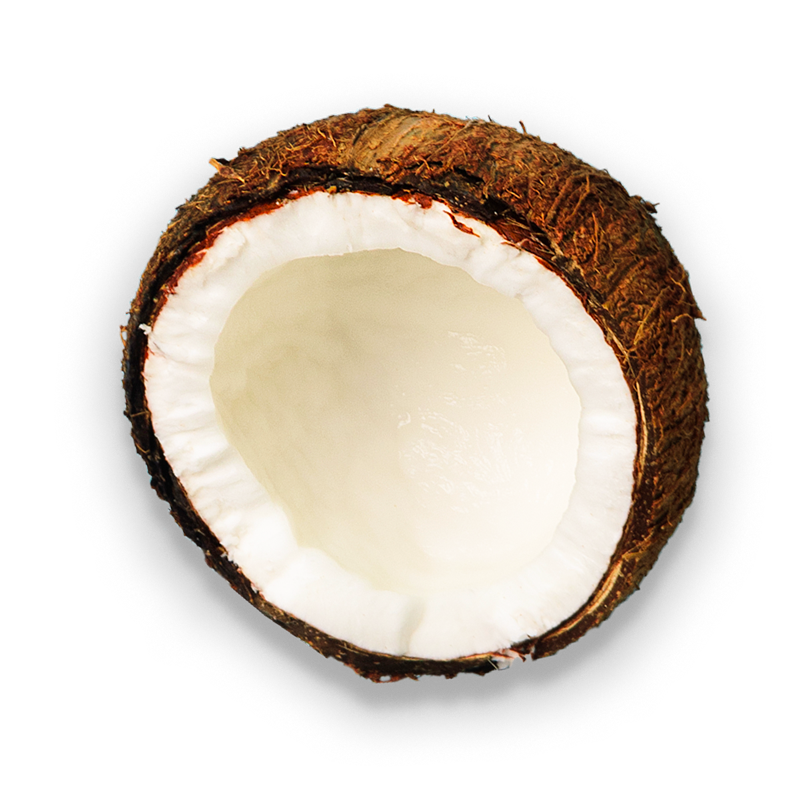
\includegraphics[width=2in]{coconut.png}
%     \caption{this is a coconut}
%     \label{test image coconut}
% \end{figure}

% image across two columns
% \begin{figure*}[!ht]
%     \centering
%     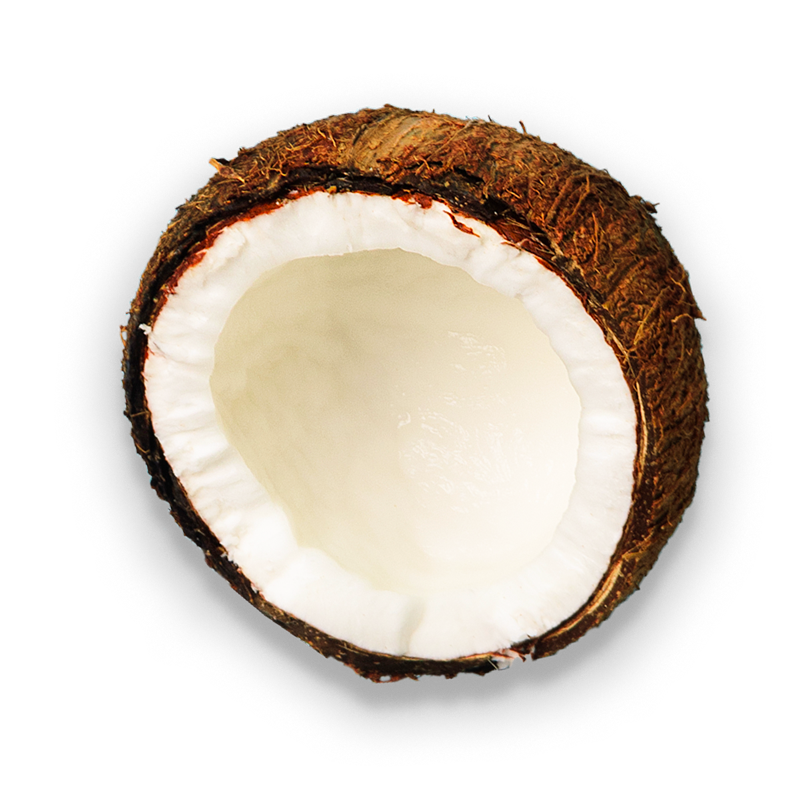
\includegraphics[width=3in]{coconut.png}
%     \caption{this is a coconut}
%     \label{coconut}
% \end{figure*}

\begin{figure*}[!ht]
    \centering
    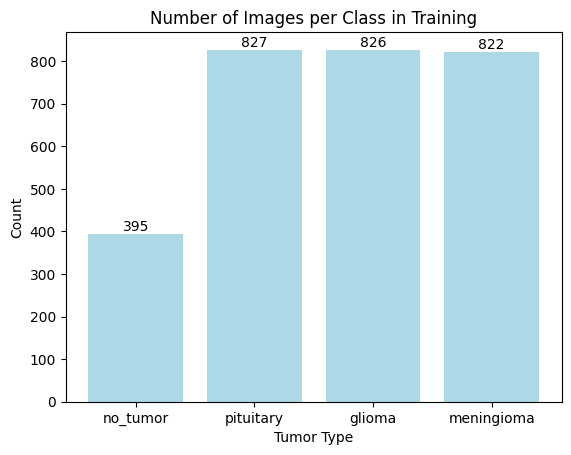
\includegraphics[width=4in]{ImagesPerClassTraining.png}
    \caption{\large Number of images per class in the training dataset}
    \label{Number of images per class in the training dataset}
\end{figure*}

\begin{figure*}[!ht]
    \centering
    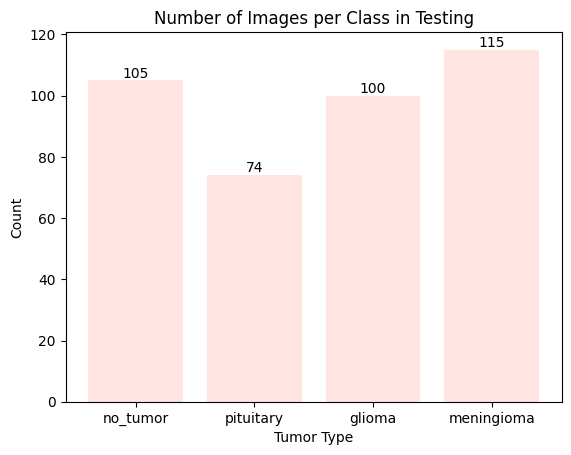
\includegraphics[width=4in]{ImagesPerClassTesting.png}
    \caption{\large Number of images per class in the testing dataset}
    \label{Number of images per class in the testing dataset}
\end{figure*}

\begin{figure*}[!ht]
    \centering
    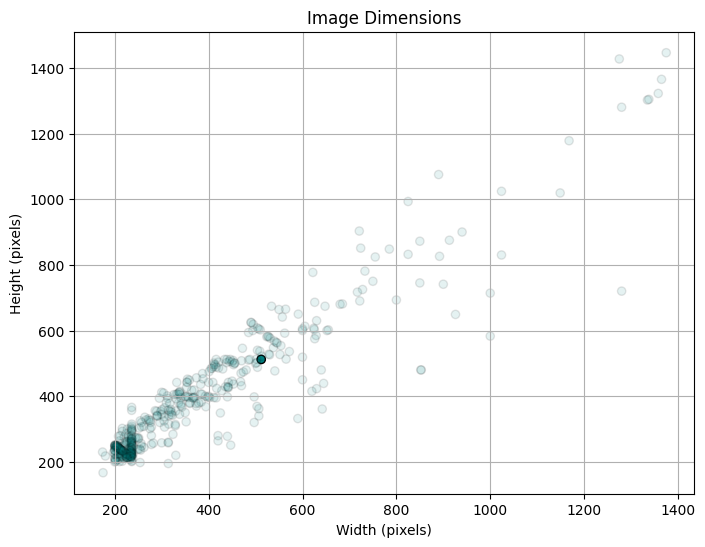
\includegraphics[width=4in]{ImageDimensions.png}
    \caption{\large Dimensions of the images in the dataset}
    \label{Dimensions of images in the dataset}
\end{figure*}

As we can see in Figure 1, there is an even distribution of images among each class (~825), except for the no tumor class (395). This is because the images without tumors have much less variance. It should be much easier for the model to detect tumor vs no tumor, so we do not expect the lower number of images in the no tumor class to have a negative effect on the model's ability to classify images as such. However, if we do see poor results in that classification specifically, we can try changing all classes to train on 395 images, to see if that helps with the class-specific overfitting.

In our test dataset seen in Figure 2, we have a much more uneven distribution among each class. This of course won't affect our model's ability, since it is not being trained on this data, but some results could be skewed considering the relatively low number of pituitary images. It could be useful to test against more pituitary imagery to ensure the model can handle all variations of scans. We could perform data augmentation and create more data by rotating, zooming, and flipping our existing data. Testing against more data could give us more confidence in our model, if scores remain high.

We can see in Figure 3 that our dataset is comprised of images of varying sizes. There seems to be a concentration around the 200x200 and 500x500 sizes. With this information, we know we will have to perform some image pre-processing to convert all images into the same size so the model has consistent input. A common image size is 256x256.

\section{\large Methodology (1-2 pages)}

\subsection{Feature Selection}
As mentioned in our dataset description, we don't have labels for our input features like a numerical dataset would have. We only have our images, which are technically a bunch of pixel intensity values, but it means we can't select certain features to train our dataset on. Instead, we can perform some image preprocessing and hyperparameter tuning to increase our model's accuracy.

If we look at Figure 3 again, we see all of our images have different dimensions.  As a preprocessing step, we will resize them all to be 256x256 pixels, so that our model has consistent input. We then normalize each pixel's value from its 3-channel RGB form. The resizing step is not as simple as it sounds though, we must be careful because shrinking or enlarging our images can create noise in our data. Based on future results, we might try a few different image sizes to see which is best. 

Our training dataset consists of 2870 MRI scans. If we want to give our model more images to train on, we can perform data augmentation. We can rotate, flip, and zoom our images to create 'artificial' data that will hopefully prevent overfitting and allow for our model to capture underlying patterns better. We also hope this will allow for our model to predict against a larger variety of testing data (i.e. rotated images). 

The hyperparameters of our model are crucial to achieving a good fit. In our first iteration of the model, some of the hyperparameters we chose were as follows:
%TODO --- fix table
- Image size: 256x256 pixels		- Batch size: 32		- Epochs: 30	
- Loss:  Categorical Cross Entropy 	- Metrics: Accuracy		- Dropout Rate: 0.25 and 0.50
We plan on fine tuning these parameters with techniques like grid search as we continue to optimize our model. 

\subsection{\large Early Model Development}

We have already built an early prototype of a CNN model with 4 convolutional blocks, followed by fully connected layers using Keras Sequential API. We trained our model over 30 epochs, with each epoch giving us higher accuracy, peaking at 92.56\% after the last epoch. However, when tested against our testing data, the model performs quite poorly. We see an average accuracy of 42.13\%, indicating that the model is overfitting quite heavily on the training data.

To improve upon our first model, we'll apply k-fold cross validation and tune hyperparameters such as dropout rate, number of layers/neurons, etc. We could start with some manual tuning, and eventually try implementing grid search to tune our hyperparameters. We also plan to use transfer learning to reduce the number of learned parameters and implicitly filter irrelevant features, which can greatly reduce overfitting risks. Going forward, we'll use PyTorch, which gives more flexibility in controlling forward pass, backpropagation, and optimization, to develop a better CNN model.


\section{\large Experimental Results (2 pages)}

\section{\large Evaluation (1-2 pages)}

\section{\large Conclusion (1/2 page)}

\section{\large Our Team (1 page)}
The link to our GitHub repository for this project can be foun at: https://github.com/Coco501/Neural-Networks-for-Neural-Tumors

project roadmap? 
%TODO --- roadmap?

\subsection{\large Roles and Contributions}

Joe: As the team leader, Joe has taken charge of organizing meetings, assigning tasks, and the general oversight over the project. In the coming weeks, Joe will be focusing on Exploratory Data Analysis, Literature Review, and Model Optimization. 

Nam: Nam took charge of making the first prototype of our model. Having this model as a starting and reference point is absolutely crucial in the development of subsequent models. In the next few weeks, Nam will be researching different frameworks and libraries to develop other CNN models to see which best fit our dataset.

Jonathan: Jonathan took charge of literature review and researched techniques that can be implemented to the model. In the next few weeks, Jonathan will be focusing on writing the proposed methodology for the final report.

Richard: Richard has completed an article for literature review. Over the coming weeks, he will work towards exploratory data analysis (EDA) and preparing the dataset for analysis through data pre-processing.

Aryan: Aryan completed a literature review and analyzed research papers to identify techniques we can use to address the models overfitting. In the next few weeks Aryan will continue working to improve the models accuracy while also working on documentation and reports. 

\begin{thebibliography}{00}

\bibitem{Khan2021}
H. A. Khan, W. Jue, M. Mushtaq, and M. U. Mushtaq, “Brain tumor classification in MRI image using convolutional neural network,” *Math. Biosci. Eng.*, 2021. 

\bibitem{Farooq2017}
A. Farooq, S. Anwar, M. Awais, and S. Rehman, “A deep CNN based multi-class classification of Alzheimer's disease using MRI,” in *Proc. IEEE Int. Conf. Imaging Syst. Tech. (IST)*, 2017, pp. 1-6. 

\bibitem{Seetha2018}
J. Seetha and S. S. Raja, “Brain tumor classification using convolutional neural networks,” *Biomed. Pharmacol. J.*, vol. 11, no. 3, p. 1457, 2018.

\bibitem{Sartaj2020}
Sartaj. “Brain Tumor Classification (MRI).” Kaggle, 24 May 2020, www.kaggle.com/datasets/sartajbhuvaji/brain-tumor-classification-mri. 

\bibitem{Kumar2014}
R. S. Kumar and M. Karnan, “Review of MRI image classification techniques,” *Int. J. Res. Stud. Comput. Sci. Eng.*, vol. 1, no. 1, pp. 21-28, 2014. 

\bibitem{Hasan2019}
A. M. Hasan, H. A. Jalab, F. Meziane, H. Kahtan, and A. S. Al-Ahmad, “Combining deep and handcrafted image features for MRI brain scan classification,” *IEEE Access*, vol. 7, pp. 79959-79967, 2019. 

\bibitem{Meier2020}
R. Meier, A. P. de Mortanges, R. Wiest, and U. Knecht, “Exploratory analysis of qualitative MR imaging features for the differentiation of glioblastoma and brain metastases,” *Front. Oncol.*, vol. 10, p. 581037, 2020.

\end{thebibliography}


\end{document}